% Asset ID: A22NormalDistributionTIKZ-003
% Source: Phase 1 Worked Example 12 and A22-HT adjacent content
% Related lesson section: Core Theory Part 8
% Purpose: Two-tailed critical region for a normal mean test
\documentclass[tikz,border=8pt]{standalone}
\usepackage{amsmath}
\usepackage{tikz}
\usetikzlibrary{arrows.meta,calc}
\begin{document}
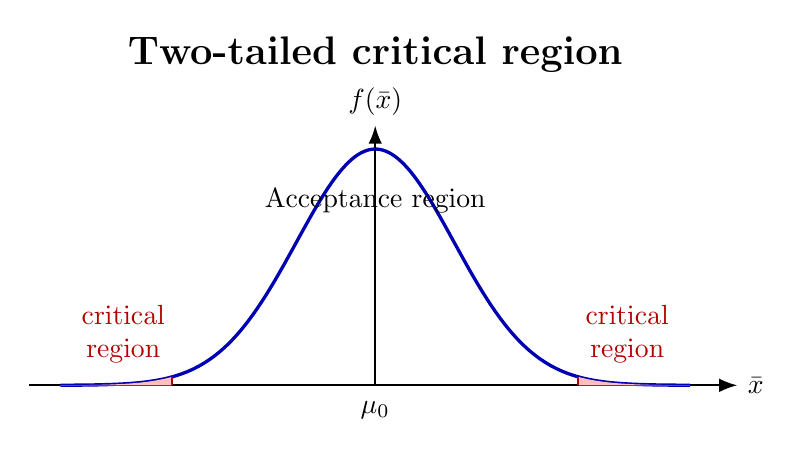
\begin{tikzpicture}[x=1cm,y=1cm,>=Latex]
\node[font=\Large\bfseries] at (0,4.2) {Two-tailed critical region};
\draw[->, thick] (-4.4,0) -- (4.6,0) node[right] {$\bar{x}$};
\draw[->, thick] (0,0) -- (0,3.3) node[above] {$f(\bar{x})$};
\draw[very thick, blue!70!black, domain=-4:4, samples=250] plot (\x,{3*exp(-0.5*\x*\x)});
\fill[red!25, domain=-4:-2.58, samples=100] plot (\x,{3*exp(-0.5*\x*\x)}) -- (-2.58,0) -- (-4,0) -- cycle;
\fill[red!25, domain=2.58:4, samples=100] plot (\x,{3*exp(-0.5*\x*\x)}) -- (4,0) -- (2.58,0) -- cycle;
\draw[dashed, thick, red!70!black] (-2.58,0) -- (-2.58,{3*exp(-0.5*2.58*2.58)});
\draw[dashed, thick, red!70!black] (2.58,0) -- (2.58,{3*exp(-0.5*2.58*2.58)});
\draw[dashed, thick] (0,0) -- (0,3);
\node[below] at (0,-0.08) {$\mu_0$};
\node[red!70!black, align=center] at (-3.2,0.65) {critical\\region};
\node[red!70!black, align=center] at (3.2,0.65) {critical\\region};
\node[align=center] at (0,2.35) {Acceptance region};
\end{tikzpicture}
\end{document}
